
\documentclass[titlepage,a4paper]{article}

\usepackage{a4wide}
\usepackage[colorlinks=true,linkcolor=black,urlcolor=blue,bookmarksopen=true]{hyperref}
\usepackage{amsmath}
\usepackage{bookmark}
\usepackage{fancyhdr}
\usepackage[spanish]{babel}
\usepackage[utf8]{inputenc}
\usepackage[T1]{fontenc}
\usepackage{graphicx}
\usepackage{float}
\pagestyle{fancy} % Encabezado y pie de página
\fancyhf{}
\fancyhead[L]{TP1S - Max Mustermann}
\fancyhead[R]{Algoritmos y Programación III - FIUBA}
\renewcommand{\headrulewidth}{0.4pt}
\fancyfoot[C]{\thepage}
\renewcommand{\footrulewidth}{0.4pt}

\begin{document}
\begin{titlepage} % Carátula
	\hfill
\includegraphics[width=6cm]{img/logofiuba.jpg}
    \centering
    \vfill
    \Huge \textbf{Trabajo Práctico 2 - Algohoot\\ Primera Entrega}
    \vskip2cm
    \Large [7507/9502] Algoritmos y Programación III\\
    Curso 1\\ % Curso 1 para el de la tarde y 2 para el de la noche
    Primer cuatrimestre de 2020 
    \vfill
    \begin{tabular}{  l  } % Datos del alumno
      Kovnat, Leoni, Locatelli, Rosenblatt y Venglar. %Orden alfabético
  	\end{tabular}
    \vfill
    \vfill
\end{titlepage}

\tableofcontents % Índice general
\newpage

\section{Introducción}\label{sec:intro}
El presente informe reune la documentación de la solución del segundo trabajo práctico de la materia Algoritmos y Programación III que consiste en implementar el juego de trivia Kahoot, denominado por nosotros como Algohoot, utilizando los conceptos del paradigma de la orientación a objetos vistos hasta ahora en el curso.

\section{Supuestos}\label{sec:supuestos}
% Deberá contener explicaciones de cada uno de los supuestos que el alumno haya tenido que adoptar a partir de situaciones que no estén contempladas en la especificación.

\subsection{Puntaje Negativo}

Un jugador admite puntaje negativo si responde mal una pregunta con penalidad y tiene puntaje nulo. 

\section{Diagramas de Clases}\label{sec:diagramasdeclase}
% Uno o varios diagramas de clases mostrando las relaciones estáticas entre las clases.  Puede agregarse todo el texto necesario para aclarar y explicar su diseño. Recuerden que la idea de todo el documento es que quede documentado y entendible cómo está implementada la solución.

Dejamos a continuación el diagrama de clases que representa las relaciones establecidas hasta el momento:

\begin{figure}[H]
\centering
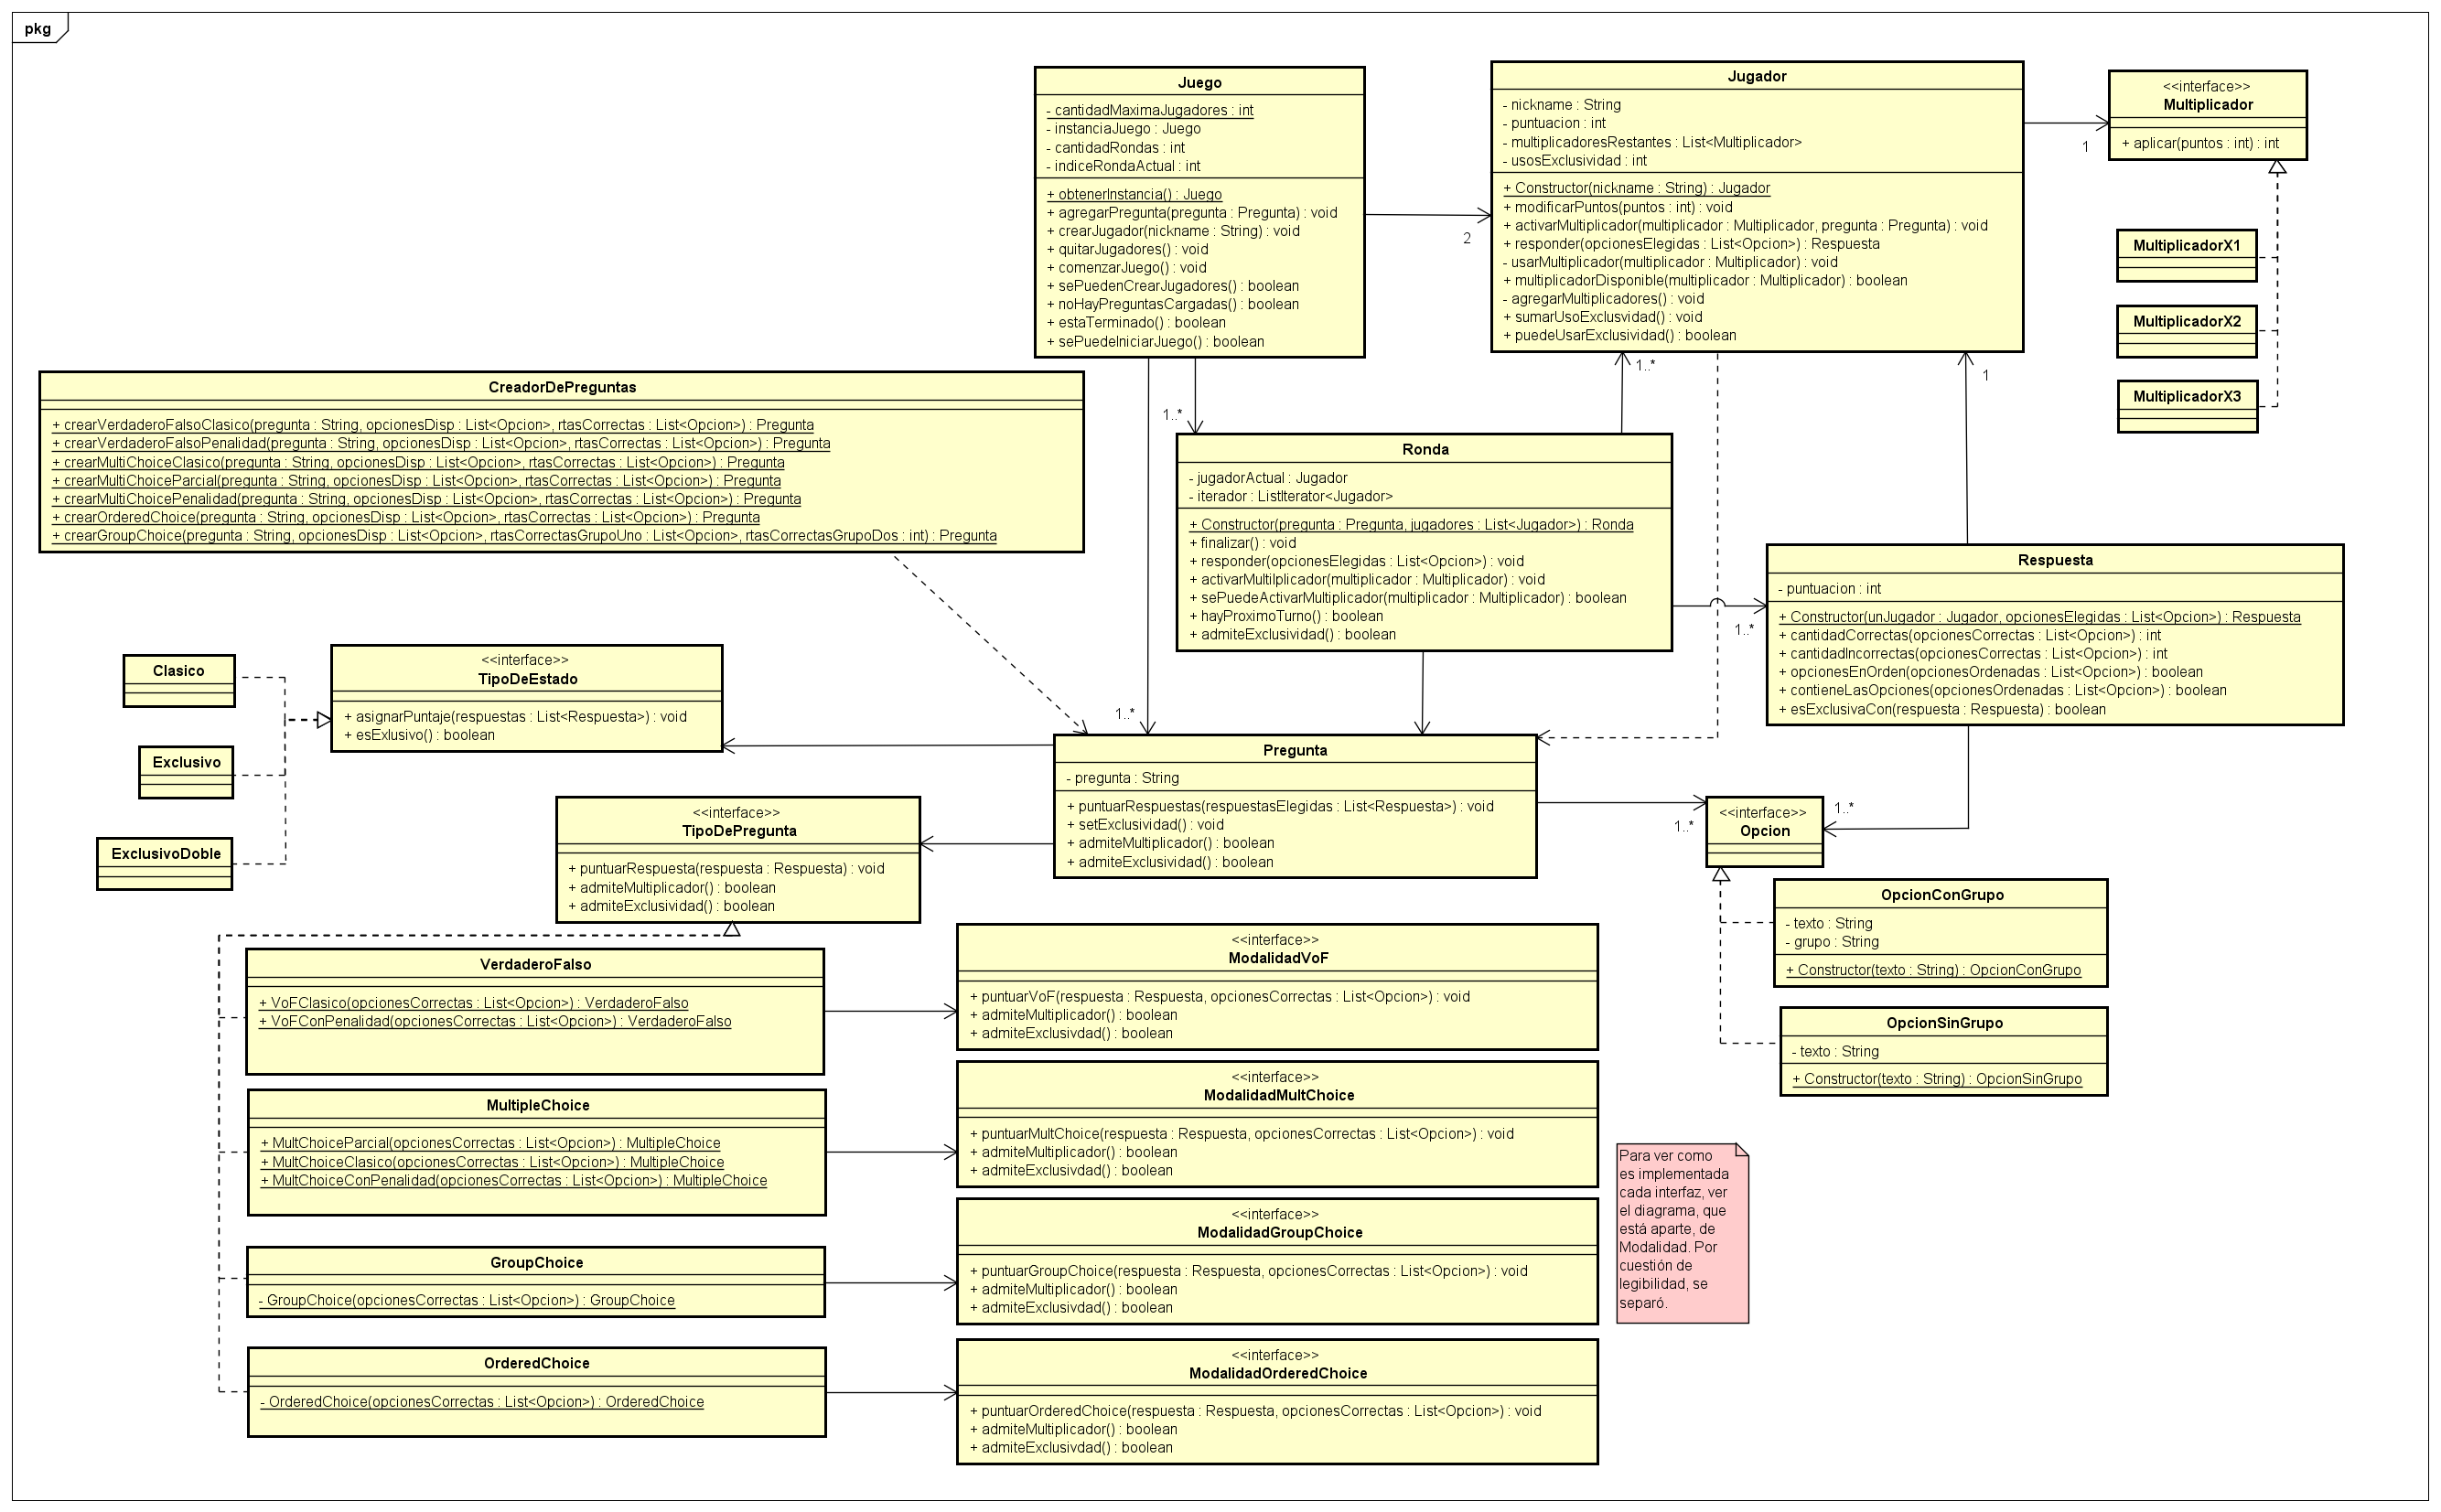
\includegraphics[width=0.8\textwidth]{img/UMLClases1.png}
\caption{\label{fig:class01}Diagrama de clases.}
\end{figure}

\section{Diagramas de Secuencia}

Dejamos a continuación los diagramas de secuencia que muestran las acciones más importantes:

\begin{figure}[H]
\centering
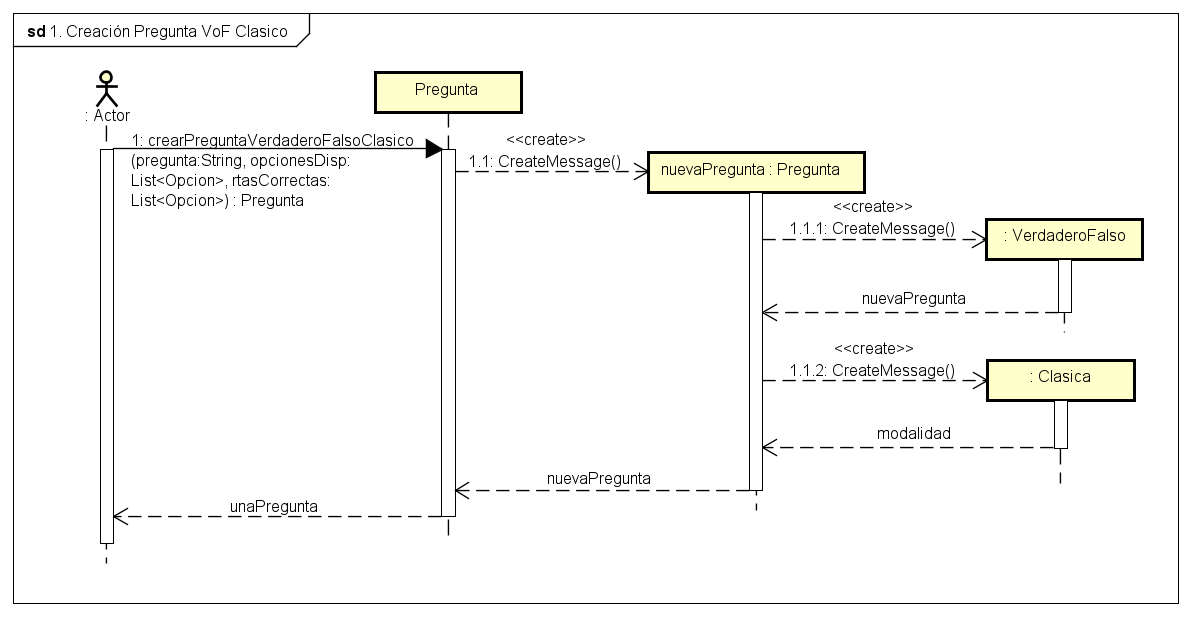
\includegraphics[width=0.8\textwidth]{img/UMLSeq2.png}
\caption{\label{fig:class01}Creación de la instancia de Pregunta.}
\end{figure}

\begin{figure}[H]
\centering
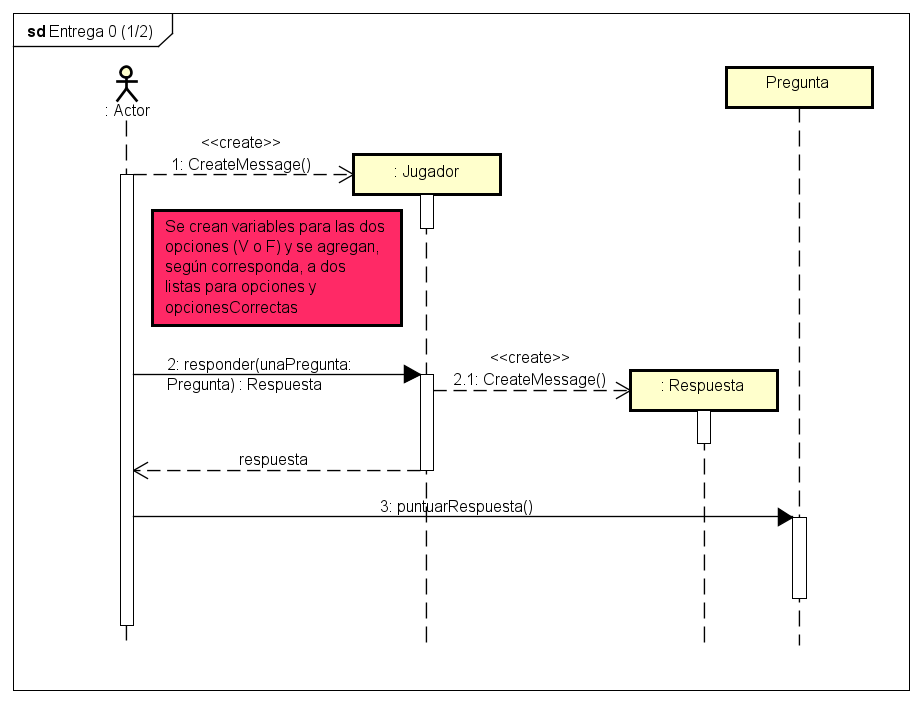
\includegraphics[width=0.8\textwidth]{img/UMLSeq3.png}
\caption{\label{fig:class01}Evaluado de respuestas (1/2).}
\end{figure}

\begin{figure}[H]
\centering
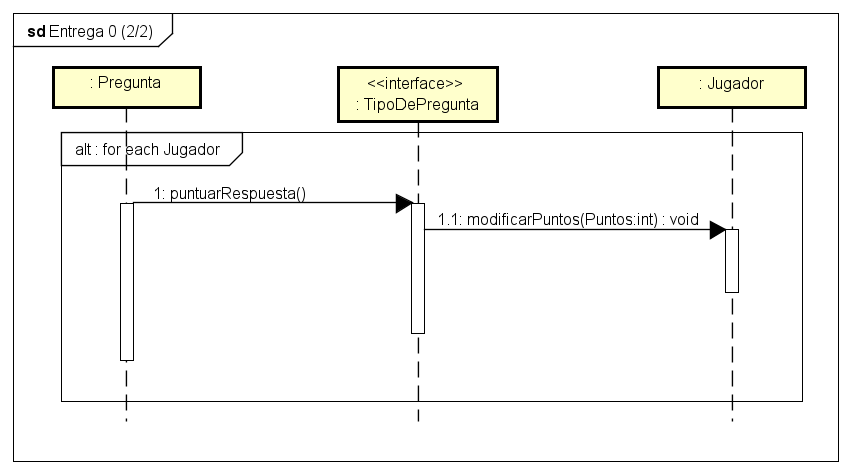
\includegraphics[width=0.8\textwidth]{img/UMLSeq4.png}
\caption{\label{fig:class01}Evaluado de respuestas (2/2).}
\end{figure}

\section{Diagrama de Paquetes}
% Explicación concisa del diseño general del trabajo.

No se solicita para esta entrega.

\section{Diagramas de Estados}
% Explicación concisa del diseño general del trabajo.

No se solicita para esta entrega.

\section{Detalles de implementación}
% Explicaciones sobre la implementación interna de algunas clases que consideren que puedan llegar a resultar interesantes.

\subsection{Como se contesta una pregunta}

Una vez creada una Pregunta usando varios objetos Opcion, y creado uno o varios objetos Jugador, estos últimos generan cada uno un objeto Respuesta (mediante el método responder) el cual contiene una referencia al propio Jugador y una lista de (algunos o todos) los objetos Opcion usados en Pregunta. Esta lista corresponde a las opciones que el correspondiente Jugador eligió.

Después de eso se le da a Pregunta, mediante el método puntuarRespuesta, una lista compuesta de las Respuestas creadas por cada uno de los objetos Jugador. Entonces, puntuarRespuesta hace lo siguiente:
\begin{enumerate}
\item Itera por todas las Respuestas de la lista, y delega la verificación de las mismas, así como la correspondiente asignación de puntaje para cada Jugador, al objeto Estado (asociado a Pregunta), que a su vez se lo delega a TipoDePregunta, que a su vez se lo delega a Modalidad.
\item Por último, Modalidad se encarga de comparar los objetos Opcion de la pregunta con los objetos Opcion de la Respuesta, y asigna los puntos correspondientes al Jugador asociado a esa respuesta, usando el método puntuarRespuesta.
\end{enumerate}

El hecho de que cada objeto Pregunta y TipoDePregunta tenga objetos asociados que definan el comportamiento del mismo (Pregunta tiene Estado y TipoDePregunta, mientras que TipoDePregunta tiene Modalidad), corresponde al patrón de diseño Strategy.


\section{Documentación}

\subsection{Jugador}
Cada instancia de Jugador tendrá un nombre, puntos y un multiplicador asociados al mismo. Se inicializa con puntaje en cero y nombre recibido por parámetro. Esta clase posee los métodos:
\begin{enumerate}
\item \begin{verbatim}public Respuesta responder(List<Opcion> opcionesElegidas);\end{verbatim} Recibe una lista de opciones seleccionadas por el jugador durante el turno vigente para crear y devolver una instancia de Respuesta que posee el nombre del jugador y dichas opciones. 
\item \begin{verbatim}public void modificarPuntos(int puntos);\end{verbatim} Este método recibe el número de puntos que se le deben añadir al jugador, ya sean positivos o negativos. 
\end{enumerate}

\subsection{Pregunta}
Esta clase está formada por el texto literal de la pregunta, la lista de opciones disponibles, la lista con las opciones correctas su tipo y su modalidad.

Las preguntas se clasificarán por:\\

\begin{tabular}{l}
Tipo: "Verdadero o Falso"$ $ y "Multiple Choice" $ $(hasta el momento).\\
Modalidad: Clásica, con puntaje Parcial y con Penalidad.\\\\
\end{tabular}

Por cada turno, la pregunta en curso recibirá una lista de respuestas emitidas por cada jugador. \\

\begin{enumerate}
\item \begin{verbatim}public static Pregunta crearPreguntaTipoYModalidad\end{verbatim} \begin{verbatim} (String pregunta, List<Opcion> opcionesDisponibles, List<Opcion> respuestasCorrectas);\end{verbatim}
 Recibe la pregunta literal, una lista de opciones seleccionadas por el jugador durante el turno vigente y la lista de opciones correctas, para crear y devolver una instancia de Pregunta del tipo y modalidad especificados.
\item \begin{verbatim}
public void puntuarRespuesta(List<Respuesta> respuestasElegidas);\end{verbatim}
Este método recibe una lista con las respuestas elegidas por el jugador y por cada una se evalúa su veracidad, para determinar si se debe modificar el puntaje del jugador.
\end{enumerate}


\section{Excepciones}
% Explicación de cada una de las excepciones creadas y con qué fin fueron creadas.

\begin{description}
\item[Exception] COMPLETAR
\end{description}

\end{document}